%!TEX root = ../main.tex
\newacronym{4d}{4D}{four dimensional}
\newacronym{3d}{3D}{three dimensional}
\newacronym{2d}{2D}{two dimensional}
\newacronym{crl}{CRL}{crown-rum length}
\newacronym{hc}{HC}{head circumference}
\newacronym{itk}{ITK}{Insight Segmentation and Registration Toolkit}
\newacronym{dicom}{DICOM}{Digital Imaging and Communications in Medicine}

Medical fetus diagnostics involves in most cases ultrasound imaging and visualization \cite{Viola2013}. The low costs and the fact that there is no radiation involved leads to a growing interest in this medical recording process and the involved visualization techniques \cite{Huang2017}. \gls{3d} ultrasound has become a major field of research since the early 1980s \cite{Correa2010}. Nowadays also \gls{4d} ultrasound imaging is possible where the \gls{3d} images are recorded in real time and represented as moving images \cite{Yagel2007}. Yagel et.al. state that \gls{3d} and \gls{4d} ultrasound scanning devices are available in many centers where fetal diagnostics is performed \cite{Yagel2007}.  The diagnostics of the fetus growth is one of the major fields where \gls{2d} and \gls{3d} as well as 4D ultrasound techniques are used \cite{Moeglin2005}. Measuring the growth of the fetal organs in addition to the overall development is a very important factor for the healthy development of the fetus \cite{Moeglin2005}. Ultrasound is widely used to measure e.g. the growth of the fetal lungs \cite{Moeglin2005}. Having a look at the general growth development of the fetus is very important for the early detection of abnormalities in development or other complications during the pregnancy \cite{Whitworth2014}.\newline\newline

Beside the organs the overall growth of the fetus is also of a great interest. Important variables are for example the \gls{crl} and the \gls{hc} \cite{Loughna2009}. There are also other measurements used to predict the fetal growth using circumferences like the head circumference or the abdominal circumference. Those circumferences are, when using 2D images not easy to describe and measure. Different approaches may be used depending on multiple measurements \cite{Loughna2009}. According to Schild et.al another interesting measurement is also the femur length because in combination wit the \gls{hc} it may be used to calculate the predicted weight of the fetus \cite{Schild2000FetalUltrasound}. Overall it can be said that measuring the fetus during the pregnancy is a very important but in some cases very tedious to perform. That is the reason why transforming the fetus to a standardized position like a T shaped position would be useful. The measurements of the limbs would be much easier and easy comparable over time. Overall height could be estimated automatically as well as the span of the arms. It can be said that a \gls{3d} visualisation and transformation as well as a guided measurement tool would be useful.

\section{Problem definition and research questions}

Transforming of given data into a specific position requires somehow knowledge of the given data in order to perform the task \cite{Singh2004}. This knowledge might be included in the dataset given or may be the result of some interaction with the user. In order to somehow anatomically correctly model a fetus into a new formation the skeleton or an abstract version of the skeleton may be used. The key points of the skeleton which have to be correctly placed in the data are the joints. The joints are the points where the different parts of the limbs rotate around in order to generate new posture of the given body. Having figured out how to incorporate the armature into the data the next step is to transform it.\newline

The transformation of the fetus has to be done in a way that the result is a fetus with his or her arms in a horizontal line and the legs shall be straight and in parallel. One may imagine the famous image of Leonardi Da Vinci named the vitruvian man where a man is drawn in a perfect T-position. Figure \ref{fig:vitruvianMan} shows the famous picture. The problem at this step is to find out how the different parts have to be transformed in order to bring them into that special shape. 

\begin{figure} [!htb]
    \centering
	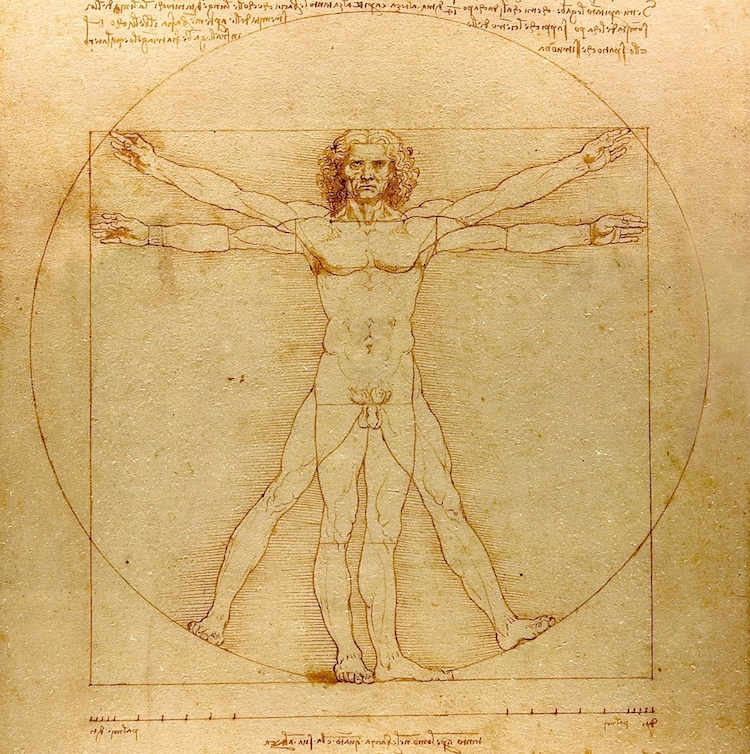
\includegraphics[width=10cm]{content/images/vetruvianMan.png}
	\caption{The vitruvian man by Leonardo da Vinci \cite{daVinci1492TheMan}.} 
	\label{fig:vitruvianMan}
\end{figure}

\section{Overview of the aimed solution}
Having a look at the clinical procedure when performing fetus analysis there is definitely a room for improvement. The first step is to acquire the data of the fetus. This step may be one of the most important ones because it determines the completeness and the quality of the fetal data. Therefore this step should already be guided and in a way that the clinical personal is able to perceive the data which is already acquired and where some additional data may be useful. In order to be able to capture and visualize a fetus during the ultrasound session the compounding feature introduced by Viola et. al. may be of a great interest \cite{Viola2013}.\newline

After the recording of the data the processing of it is the next step. The idea is that the fetus is processed in a way that it can be presented in a T-position. This position enables different kinds of measurements and enables a clear view of the limbs as well as the head. At some point one might consider the interaction with the operator of the program useful and fruitful and this might be one of those. The process of interactively reforming the fetus data into a given position requires first the integration of a so called armature into the data. The armature describes the joints and bones of the skeleton in an abstract way. Some points may be moved into the data automatically but it might be a better solution to ask the operator of the system to define some key points and let the machine describe the rest of the data.\newline

After having the armature embedded in the data the weighting has to be done. Weighting means that the program has to calculate the affinity of voxels to segments of the armature. This step can be done completely automatically. After the volume data has been linked to the armature the transformation can be done. The transformation analyses the position of the armature and moves each part of the limbs of the fetus against others in respect to the joints. The angles which have to be used when applying the rotations in 3D space may be calculated and applied automatically. The result should be a representation of the acquired fetus data showing the whole fetus at a glance in a T-position.\newline

The end results may also include the standardized measurements automatically taken by the machine. The introduction of this system may also lead to the development of new measurements which take the whole span from finger to finger or the size of the fetus from head to toe. The representation of a fetus in a standardized way also enables the data to be comparable in means of time or inter specimen differences.

\section{Requirements}

Loading the volumetric data of the fetal ultrasound analysis into the program shall be rather easy and the system should support well-known file formats used in medicine like the file formats used by the \gls{itk}. Another approach would be to use the file format called \gls{dicom} which is commonly used in clinical application or generally when working with medical data.\newline

If the source is an ultrasound investigation preprocessing to remove artefacts might be applied. The processing may include filtering to get rid of artefacts induced by for example the mother fluid or interactions with the tissue which the sound wave has to cross in order to perceive the fetus. In ultrasound images the data which represent the fetus normally have a specific range of values, therefore a threshold may be applied. If the further processing steps also assume or require that the data only includes the fetus and nothing else a largest connected component analysis should also be performed. This step searches, like the name says the largest connected component in a \gls{3d} volumetric dataset which should be the fetus. The rest of the image may be declared as artefacts or not relevant and can be neglected.\newline

The solution shall provide an interface where the user is able to interact with the system. The system shall provide an "easy to use" graphical desktop where the interaction is carried out. A  pipeline that guides thought the different steps of the transformation would be appreciated. In general the aim is to minimize the input needed from the end-user and shift the focus on automatic processing of the data. One step where interaction is very likely to be used is the rigging of the data. Finding a skeleton or incorporating a predefined armature into the data may be out of scope of this thesis and therefore user interaction is thinkable. The integration of the armature into the data should not take too much time and has to be very easy to carry out. The armature or skeleton is a preset where all the joints and the bones are already defined and only have to be put at the right spot inside of the volume. This step can be done by using a simple drag and drop interaction in a \gls{3d} view of the model. The user therefore has to be somehow familiar with the navigation in volume explorer and should have some kind of anatomical knowledge.\newline

Once the armature is at the right spot the weighting of the voxels has to be performed. This step is also called skinning, because the data is attached to the armature like a skin. This step should also work automatically but user interaction may be included in order to review and check the assignment. The assignment of the data to specific bones may be overwritten by the operator in order to deliver better results. The program should evaluate and preferably also visualize the belongingness of the voxels to the armature parts.\newline

The main step of the processing steps introduced in this thesis namely the T-transformation should be performed completely automatically and the results should also be exportable for further visualization and analysis. Transforming the data should not require any further input or interaction with the user. The data and the armature should be the only input for the module handling the transforming process. The end result although should again be inspectable and there should be some possibilities to automatically measure the fetus. It can also be thought of automatically display the main measurements like the span from fingertip to fingertip and from head to toe.  
